\usetikzlibrary{arrows.meta,calc}
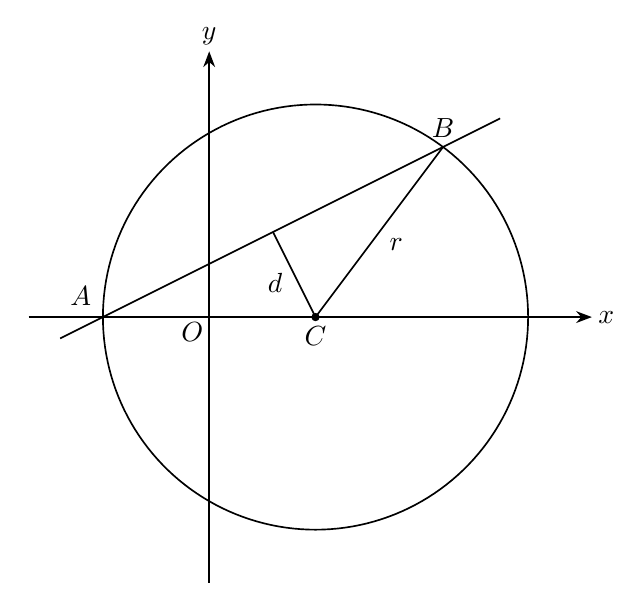
\begin{tikzpicture}[x=1.35cm,y=1.35cm,line width=.6pt,font=\normalsize,>=Stealth]
\def\rad{2}
\coordinate (O) at (0,0);
\coordinate (C) at (1,0);
\coordinate (A) at (-1,0);
\coordinate (B) at (2.2,1.6);
\coordinate (Df) at (0.6,0.8);
\coordinate (La) at (-1.4025,-0.2012);
\coordinate (Lb) at (2.7367,1.8683);
\draw[->] (-1.7,0)--(3.6,0) node[right,inner sep=0pt,xshift=2pt] {$x$};
\draw[->] (0,-2.5)--(0,2.5) node[above,inner sep=0pt,yshift=2pt] {$y$};
\draw plot[domain=0:360,samples=181,variable=\t] ({1+\rad*cos(\t)},{\rad*sin(\t)});
\draw (La)--(Lb);
\draw (C)--(Df);
\draw (C)--(B);
\fill (C) circle (1.5pt);
\node[above left,inner sep=4pt] at (A) {$A$};
\node[above,inner sep=0pt,yshift=3pt] at (B) {$B$};
\node[below,inner sep=0pt,yshift=-3pt] at (C) {$C$};
\node[anchor=center,inner sep=0pt] at (-0.16,-0.14) {$O$};
\node[anchor=center,inner sep=0pt] at (0.62,0.32) {$d$};
\node[anchor=center,inner sep=0pt] at (1.76,0.68) {$r$};
\end{tikzpicture}
